\chapter{Text recognition algorithms}

Text recognition forms the basis of any complex OCR software. Its task is to transform an input image into its segmented form, with segments containing information about individual characters and their positions.

We begin this chapter by presenting various aspects that impact the quality of the input image, which we have observed to affect the results of the text recognition algorithms. To reduce the effects of these aspects, we also focus on the related task of preprocessing the input image. After that, we analyze the individual steps of the text detection process and review the existing techniques used for this purpose.
	
\section{Common obstacles of successful text recognition}

Even for human perception, the task of recognizing text in a complex document might become difficult due to various factors. Text recognition engines work similarly or, in specific cases trivial for human perception, even worse.

Common difficulties faced by text recognition algorithms have been reviewed by~\citet{preprocessAll}. These can be categorized into following major classes:

\begin{description}

\item[Font face variability] Text documents contain a lot of different fonts and styles, including different headings, body text, footer and header sizes along with bold, italics and underlined characters, differently colored fonts and even custom-made fonts. Furthermore, when it comes to handwritten text, each character is slightly different and the text contains a lot of inaccuracies. To hold the information about every possible font and style would therefore be impractical for any OCR software, and, in case of custom-made fonts or handwritten text, even impossible. Therefore, an OCR software needs to use heuristics to match the actual symbol it recognized to its expectation of the character shape. This does not always produce the desirable results. In specific cases, especially in decorative fonts or handwritten text, characters like S or 5, 0 or O and I or l are hard to distinguish even by human perception. This often results in the failure of text detection algorithm for these specific characters.

\item[Scan quality] The optimal results of image acquisition techniques, like scanning, are high-contrast images with no inaccuracies. However, the scanning process often disrupts the input image, which results in low contrast, insufficient sharpness, pixelation, noise and disruption of lines. This is usually due to a low resolution scan or human made mistakes during scanning. We use the techniques of preprocessing to try and reconstruct this error prone image into a suitable input for text recognition engines.

\item[Skew problems] Photographing or scanning an image often results in minor human made skew and rotation problems. However, most of the text recognition engines already assume the input to be properly vertically and horizontally aligned for the simplicity and time complexity of its algorithm. This deems the engines to fail on skewed images. Therefore, we attempt to deskew the input images during preprocessing with the use of deskewing techniques.

\item[Colors] To distinguish characters from the image background, OCR engines use various techniques based on the color values of the individual pixels, their contrast, brightness\ldots When it comes to monochrome one images, to determine this division of image pixels is a simple task. With colored inputs, however, many complications arise. For example, recognition of green text on a red background fails when presented to a method based on contrast. This and improved time complexity of the algorithm is the reason why images often undergo the process of binarization. 

\end{description}

These difficulties motivate the common OCR implementations to work with optimistic assumptions about documents, for example that the document has only one column, that it is not handwritten, that its lines are horizontally aligned\ldots

Several image processing techniques are used to eliminate the effects of most of
these obstacles. These techniques try to preserve as much document information as possible in quick and simple ways. Moreover, they attempt to increase the performance of OCR engines. We cover them thoroughly in the next preprocessing section.

Only once these techniques are applied to the input image is it passed to the text recognition process. Therefore, ideally, the only obstacles left for text recognition process to solve are font-faced problems.

\section{Preprocessing for OCR}

Many of the existing OCR engines already come with some kind of built-in preprocessing filter. Their problem is that they most likely do not match the exact image case and are usually very simple.

This is why the best practice is to firstly preprocess the image and then pass the result to the OCR algorithm.

In this section, we will discuss the most important image transformations that we can perform to improve the results of the OCR. 

\subsection{Scaling}

Most common methods of character recognition demand a large set of training data. Classification of newly recognized characters is then performed by comparing them to this training data.

Many popular OCR engines (e.g. Tesseract~\cite{TesseractQual}, ABBYY FineReader~\cite{ABBYYdpi}) encourage their users to use 300 dpi images. Their reason for that is pretty simple --- most of their training data were obtained from 300 dpi images, as this resolution was high enough for a clear recognition of character features, but also low enough to maintain a reasonable execution time of the algorithm. Therefore, the resolution of 300 dpi is where their recognition obtains the most accuracy~\cite{preprocessAll}. 

Obtaining a 300 dpi scan using currently available hardware is simple enough. However, if the user has already provided us with an image of a different resolution, our next step is to either upscale (if the dpi of the input image was lower) or downscale (if the dpi of the input image was higher) the image. In both cases, a technique called \emph{interpolation} is used. 

Interpolation works by using known data to estimate values at unknown points. It specifically approximates the resulting pixel's color and intensity based on the values at surrounding pixels. When downscaling, this technique therefore computes one color value for each set of pixels, which are the color values of the pixels in the new image. When upscaling, it computes color values of the new pixels by approximating the values of the old pixels around them.

This technique tries to minimize the aliasing effect of the resulting image --- so the scaled picture does not appear visibly pixelated and its edges are not jagged.

Interpolation algorithms can be grouped into two categories: \emph{adaptive} and \emph{non-adaptive}.

\emph{Adaptive methods} change the way they treat various pixels depending on what they are interpolating, specifically smooth texture vs. sharp edges. They are primarily designed to minimize the presence of interpolation artifacts in regions where they are most apparent, and they differ by the way they detect edges.

\emph{Non-adaptive} methods, on the other hand, treat all pixels equally. Their complexity depends on the number of adjacent pixels during interpolation, which is also the criterion by which the existing methods are classified~\cite{interpolation}. We present these methods in~\cref{fig:preprocessInterpolation}.

\begin{figure}[t]
\centering
{\sffamily
\begin{tabular}{cc}
Original & Nearest-neighbor Interpolation\\
 & (1 pixel) \\
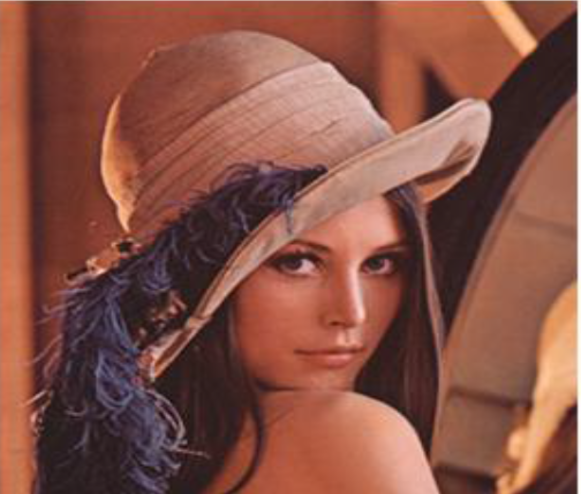
\includegraphics[width=.4\linewidth]{img/preprocessing/interp_orig.png}
&
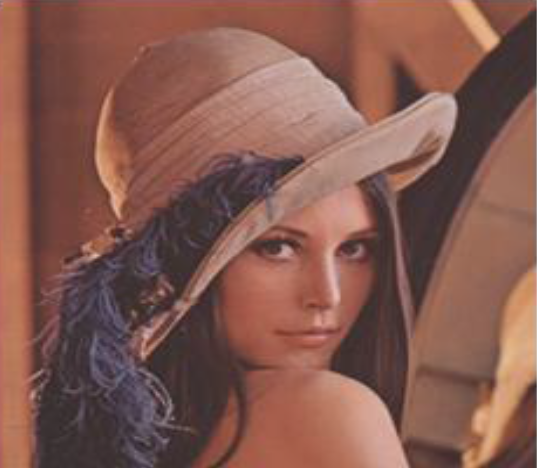
\includegraphics[width=.4\linewidth]{img/preprocessing/interp_nn.png}
\vspace{1em} \\
Bilinear Interpolation & Bicubic Interpolation \\
($2\times2$ pixels) & ($4\times4$ pixels) \\
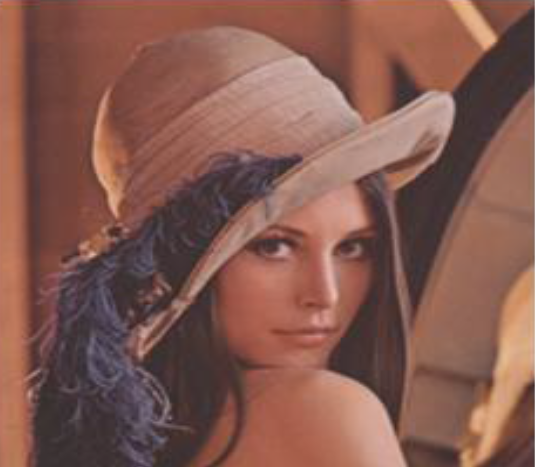
\includegraphics[width=.4\linewidth]{img/preprocessing/interp_bili.png}
&

\includegraphics[width=.4\linewidth]{img/preprocessing/interp_bicubic.png}
\end{tabular}
}
\caption{Non-adaptive methods of Interpolation}
\label{fig:preprocessInterpolation}
\end{figure}

There also exist higher order interpolations, such as \emph{Spline}, \emph{Sinc}, \emph{Lanczos} or \emph{Discrete Wavelet Transforms}~\cite{interpolation}. These consider more surrounding pixels and calculate the resulting value through more complex functions, like transforms or sampling functions. The results are more accurate than those of simple calculations at the cost of significantly more time. For the purposes of OCR, such complex and time-consuming functions are not desirable, as we are not yet working with any rotations and distortions and just need to resize the existing image.

For the best quality/time ratio, the popular decision in most cases is \emph{Bicubic Interpolation}. Although \emph{Neareast Neighbor} and \emph{Bilinear} methods are extremely fast, the results were found to be poor~\cite{interpolationComp}.

\subsection{Binarization}

To recognize characters in an image, an OCR software must distinguish the background pixels from the actual pixels that belong to the characters. The software must therefore divide all the existing pixels of the image into two groups --- a background group and a symbols group. To determine the boundary between them is a complex task when it comes to colored images, as we need to process the whole RGB information of each pixel. However, when it comes to grayscale images, we obtain only one value. Moreover, monochrome one images contain pixels of only two values --- black and white --- which make the process of finding a boundary trivial.

This is why it is beneficial for images to undergo the process of binarization, which converts images into their monochrome one form.

Many binarization algorithms work under the assumption that the input image is already in grayscale. If not, they firstly transform the image to grayscale, then apply the binarization techniques.

\subsubsection{Grayscale conversion}

\emph{Grayscale conversion} is the process of computing and assigning a gray value for each colored pixel from its attributes. There exist a few different approaches to this problem. The simplest one is the \emph{averaging approach}, which assigns each pixel the average of its R, G and B value. However, this does not really reflect the way human eye perceives colors. Our perception of colors is non-uniform --- green color is perceived more strongly than red, and red more strongly than blue. For this reason, a correction formula (often called \emph{luma}~\cite{grayscaleConv}) that weights each color component differently is used. We present these techniques in~\cref{fig:preprocessGrayscale}.

Another way to approach grayscale conversion is to represent the color based on its HSL values and convert it to its least saturated variant.

As described by~\citet{grayscaleCadik}, these exist many more algorithms approaching this problem. Most of them require more complicated computations and try to preserve attributes of the image that may be lost during the process --- like contrast or luminance.

\begin{figure}[t]
\centering
{\sffamily
\begin{tabular}{ccc}
Original & Averaging technique & Luma correction \\
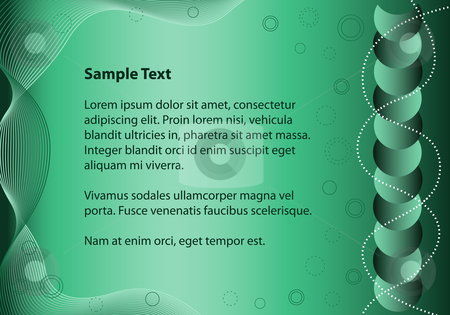
\includegraphics[width=.28\linewidth]{img/preprocessing/grayscale_orig.jpg}
&
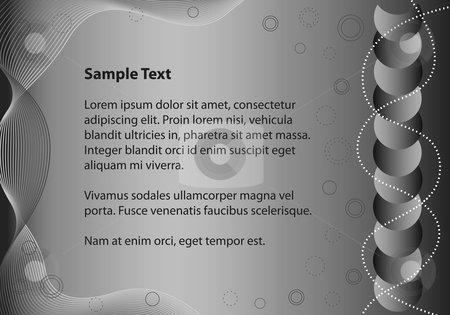
\includegraphics[width=.28\linewidth]{img/preprocessing/grayscale_avg.png}
&
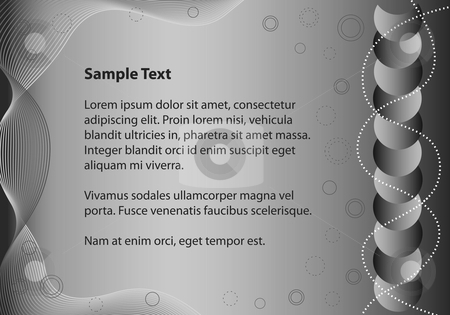
\includegraphics[width=.28\linewidth]{img/preprocessing/grayscale_luma.png}
\end{tabular}
}
\caption{Comparison of grayscale techniques}
\label{fig:preprocessGrayscale}
\end{figure}

\subsubsection{Threshold-based binarization}
Once the image is in grayscale mode, the next step is to binarize it. Binarization methods work on the basis of a \emph{threshold} --- a set value that a pixel is compared to. If it is greater than the threshold, it is assumed to be white, otherwise, it is colored black. Various binarization methods differ in the way that this threshold is calculated and used.

The simplest approach to binarization is \emph{global thresholding}~\citep{globalThresh}. It works by choosing a threshold value and iterating over the whole image, comparing the value of each pixel to this threshold. If it is greater, the pixel in the resulting image will be black, otherwise white. However, as the brightness and contrast of different images vary, it is impossible to choose a threshold suitable for all images.

More complex methods that aim to correct the problems of global thresholding exist. Some of these include:
\begin{itemize}
\item Otsu's method for global threshold estimation~\citep{otsu}
\item Local-thresholding methods~\citep{localOtherBin}:
\begin{itemize}
\item Niblack method
\item Bernsen method
\item Sauvola method
\end{itemize}
\end{itemize}

Otsu's method statistically computes a global threshold by a dynamical classification of image pixels into background and foreground pixels. Although simple and easy to implement, but, as any global method, it is inherently unable to fix high variance or uneven spots in an image background. Local-thresholding methods aim to solve this issue by allowing different threshold values in different parts of the image. They differ in the way the existing thresholds are computed --- for example, Niblack's method~\citep{adaptiveBin} uses mean and standard deviation of surrounding pixels for each pixel, Sauvola Method improves it by checking for blank regions and Bernsen's method by optimizing Niblack's computations. 

Visual differences between the mentioned methods are displayed in~\cref{fig:preprocessBinarization}. Comprehensive reviews of other, more complex methods are available~\citep{localOtherBin}.

\begin{figure}
\centering
{\sffamily
\begin{tabular}{ccc}
Original scanned image &
Global Thresholding &
Sauvola Binarization \\
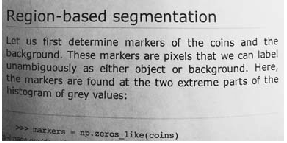
\includegraphics[width=.3\linewidth]{img/preprocessing/bin_orig.png} &
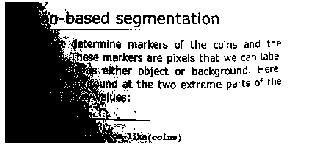
\includegraphics[width=.3\linewidth]{img/preprocessing/bin_glob.png} &
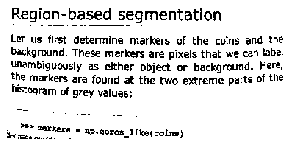
\includegraphics[width=.3\linewidth]{img/preprocessing/bin_sauvola.png}
\end{tabular}
}
\caption{Comparison of binarization method output on an unevenly lit image}
\label{fig:preprocessBinarization}
\end{figure}

\subsection{Contrast enhancement}

Another important factor that results in low-quality images is low contrast. Even human eye has a harder time recognizing images with this element. The same stands for OCR engines, as low contrast often results in possible blending of edges during recognition.

An image \emph{histogram} is used to improve this aspect. A histogram is an accurate representation of the distribution of data and, in case of image histograms, it represents the tonal distribution of an image --- x-axis stands for all available tonal levels, and y-axis represents the number of pixels for each tonal level. In colored (RGB) images, the histogram is displayed by the terms of three separate histograms --- one for each color component.

Contrast of the current color component is represented as distribution of pixel luminance values. By spreading out the most frequent intensity values of the histogram, the contrast of the image increases(~\cref{fig:preprocessContrastComparison}).

\begin{figure}[t]
\centering
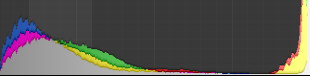
\includegraphics[width=0.4\linewidth]{img/preprocessing//histogram_low.png}
\qquad
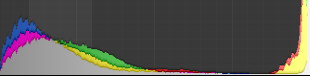
\includegraphics[width=0.4\linewidth]{img/preprocessing/histogram_high.png}
\caption{Image histogram. Left: low contrast image histogram, right: high contrast image histogram.}
\label{fig:preprocessContrastComparison}
\end{figure}

To expand the original digital values of histogram into a new distribution, different histogram spreading methods use functions of different forms. These can be either linear or non-linear, which leads to the categorization of histogram spreading methods into either \emph{linear stretching} methods or \emph{non-linear stretching} methods~\citep{linearNonStretch}.

Both types of methods have their advantages and disadvantages. Although linear methods are easier to implement, non-linear methods were shown to have given better performance~\citep{chandpa1comparative} and overall better results. Linear methods still produce satisfactory results on remotely sensed images with Gaussian or near-Gaussian histograms, and in contrary to non-linear methods, objects in the original scene do not lose their correct brightness value.

For contrast enhancement of the text, a non-linear technique called \emph{histogram equalization}~\citep{histogramEQ} is used. Is is based on transforms that depend on the probability distribution function of the histogram. Although it produces unrealistic and over-enhanced effects in photographs, the over-processing actually suits the text data. We present the effects of this widely used method in~\cref{preprocessHistogramEqualization}.

Many other more complex and complicated techniques of contrast enhancement exist. These were presented by~\citet{contrastOther} and contain techniques like CLAHE, Dynamic Stochastic Resonance and generic transforms, such as Fourier, Discrete Cosine, and Wavelet. For complex text recognition cases, CLAHE method can be used with satisfactory results.

\begin{figure}[t]
\centering
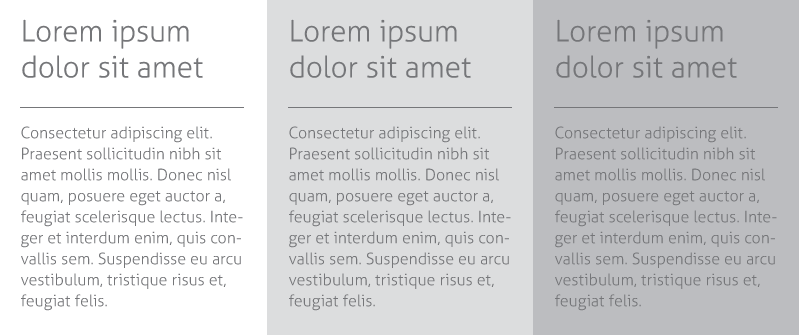
\includegraphics[width=0.4\linewidth]{img/preprocessing/contrast_low.png}
\qquad
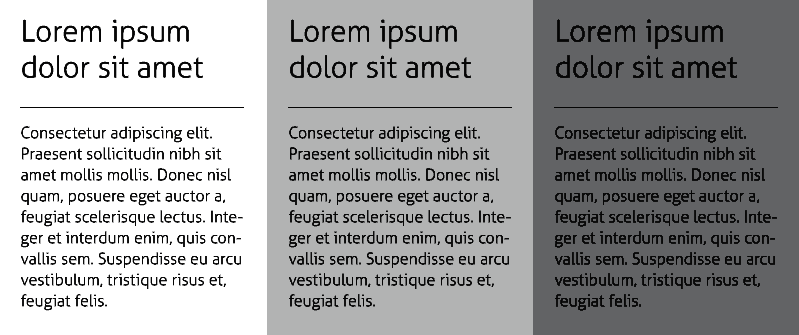
\includegraphics[width=0.4\linewidth]{img/preprocessing/contrast_high.png}
\caption{Histogram equalization. Left: original image, right: processed image.}
\label{fig:preprocessHistogramEqualization}
\end{figure}


\subsection{Deskewing}

Skewed images are probably the most common problem that many OCR engines struggle with. They usually appear when an image is scanned or photographed crookedly. 

One of the steps of OCR algorithms is \emph{page segmentation}. It is the process that decomposes a document image into elements. This division is based on vertically and horizontally aligned characters, spaces and other artifacts. We will discuss this topic thoroughly in the following chapter. For now, the important thing to know is that skewed images pass misaligned data to the OCR algorithm. This causes more errors and ultimately leads to poorer results.

There are different approaches that deal with this problem. All of these methods work (for more accurate results) after binarization of the image and generally assume the skew angle to be no more than 15$^{\circ}$. Algorithms that work on greater skew angles also exist~\citep{skewAngleDetection}. They are not as widely used, though, as most of the time, correction needs to be done on scanned documents --- which are mostly only slightly tweaked.

The most effective and popular algorithms include the following~\citep{skewBestTechniques}:
\begin{itemize}
    \item Hough Transform
    \item Projection Profile method
    \item Cross Correlation
    \item Connected Component Clustering (or \emph{Nearest Neighbor Clustering})~\citep{skewClustering}
\end{itemize}
However, worth noting are also other methods like \emph{Fourier}~\citep{fourierTransform}, Wavelet Decomposition, Radon Transform, PCP, one-pass or multi-pass skew correction, morphology algorithms\ldots.. 

The above mentioned methods differ in the way they determine the skew of the image. Hough transform applies feature extraction to the image and assigns the skew of the line with the most number of pixels to the document. Projection profile method rotates the image and finds the skew where its histogram along horizontal scan lines has the most peaks and valleys, while the cross correlation method uses this method and applies it to multiple vertical segments. Moreover, connected component clustering method is based on finding the coherency between connected components of the image and determining their common skew. We present the advantages and disadvantages of these methods in~\cref{tab:preprocessSkewProsCons}.

\begin{table}[t]
{\small
\begin{tabular}{p{5em}p{13em}p{13em}}
\toprule
\textbf{Method} & \textbf{Advantages} & \textbf{Disadvantages} \\
\midrule
Hough Transform
&
- highly effective
&
- time consuming

- cannot obtain data from graphics in an image, therefore ineffective at their presence

\\
Projection Profile method
&
- easy to implement

- works well on images with skew under 10$^{\circ}$
&

- fails at the presence of graphics

- computationally expensive

\\
Cross Correlation
&

- better time complexity than projection profile method

- needs less data with no loss in accuracy

&

- works on text areas only

- fails at the presence of graphics

\\
Connected Component Clustering
&

- satisfactory results for skew up to 20$^{\circ}$

- generally work well in non-text areas

&

- low quality images deem the method to fail

- clustering algorithm needs to be picked carefully to avoid errors

\\
\bottomrule
\end{tabular}
}
\caption{The advantages and disadvantages of different deskewing methods}
\label{tab:preprocessSkewProsCons}
\end{table}

\begin{figure}[t]
\centering
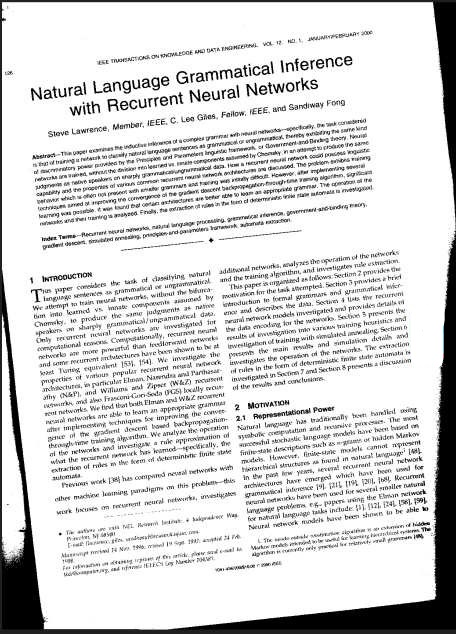
\includegraphics[height=0.25\textheight]{img/preprocessing/deskew_orig.jpg}
\qquad
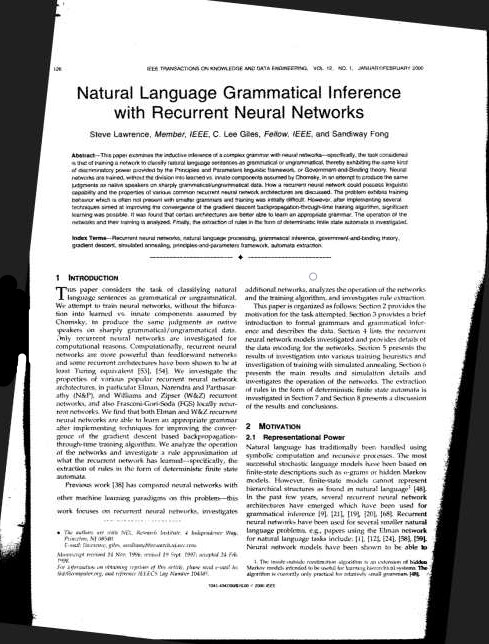
\includegraphics[height=0.25\textheight]{img/preprocessing/deskew_new.jpg}
\caption{Image deskewing illustrated. Left: original image, right: deskewed image.}
\label{fig:preprocessDeskewing}
\end{figure}

\subsection{Noise reduction}

Image noise is an usually unwanted random variation of brightness or color information in images, reminding film grain in digital cameras. It is often caused by the sensor of a scanner or a digital camera attempting to record small amounts of light. 

For OCR engines, processing noise can be quite tricky. Its presence is especially crucial during binarization and edge detection. These processes are based on the differences between the "outside" of the element and its "inside". When noise is present, it can disrupt these borders, which can often cause the failure of recognition. We present the different types of existing noise in~\cref{tab:preprocessNoiseTypes}.

\begin{table}[t]
{\small
\begin{tabular}{p{8em}p{12em}l}
\toprule
\textbf{Type} & \textbf{Description} & \textbf{Image} \\
\midrule
Salt and Pepper \par (\emph{impulse noise})
&
Randomly occurring black and white pixels caused by sharp and sudden
disturbances in image signal present in old photographs.
&
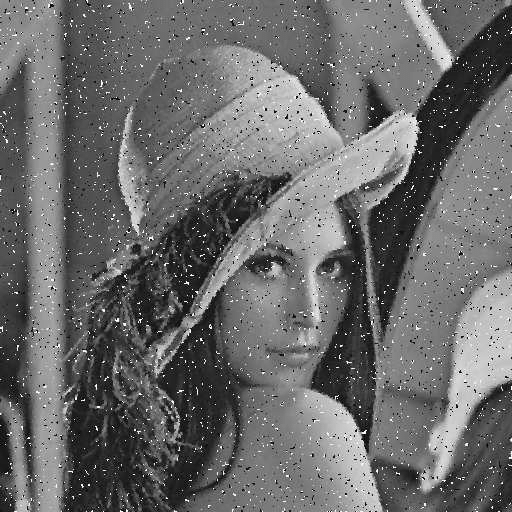
\includegraphics[width=0.3\textwidth, align=t]{img/preprocessing/noise_saltpepper.png} \\
Statistical noise 
&
Unexplained variability within an image, usually characterized by a probability density function, e.g.~\emph{Gaussian noise}, \emph{Shot noise}, \emph{Quantization noise} or film grain.
&
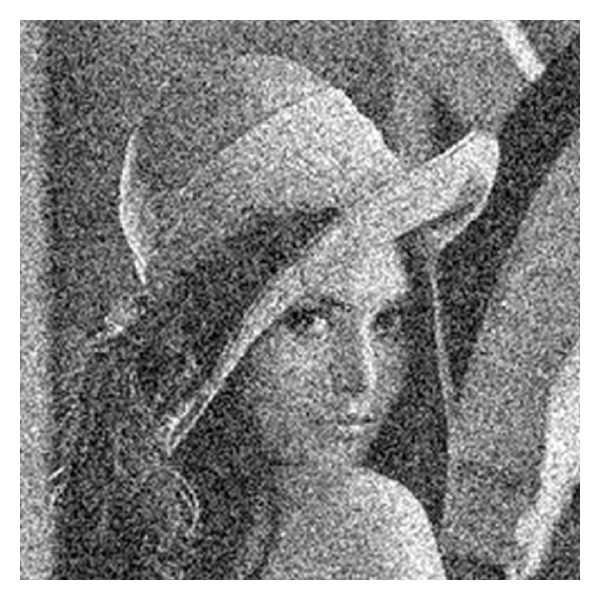
\includegraphics[width=0.3\textwidth, align=t]{img/preprocessing/noise_gaussian.jpg}\\
Other
&
E.g.~\emph{anisotropic} or \emph{periodic} noise, often found in old photographs or documents.
&
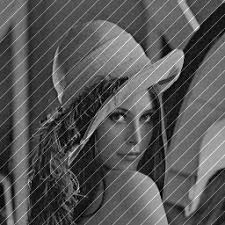
\includegraphics[width=0.3\textwidth, align=t]{img/preprocessing/noise_periodic.jpg} \\
\bottomrule
\end{tabular}
}
\caption{Different types of noise}
\label{tab:preprocessNoiseTypes}
\end{table}

When performing noise reduction, common image processing filters are used~\citep{denoisingTechniques}. These can be categorized as either linear or non-linear, depending on their linearity relationships.

\emph{Linear filtering}, such as \emph{mean filtering}, \emph{Gaussian filtering} or \emph{Wiener filtering}, is a filtering in which the value of an output pixel is a linear combination of the values of the pixels in the input pixel's neighborhood. When used for noise reduction, it works on averaging the color values of neighbour pixels, so it can help assure an averaged view of the contrast along regions of different color. This, however, rather than correcting the color of the affected pixel, results in creating an area with an average (and incorrect) color. This blurs the edges and smooths out other fine details. These filters are still widely used, though, as they require only a small amount of computations, which leads to increased speed and easy and simple implementations.

\emph{Non-linear filtering}, on the other hand, renders an output which is not a linear function of its input. They include filters like \emph{median filter} or \emph{non-local means method}~\citep{nonLocalMeans}, which are used for denoising purposes. They differ in the way the value of the current pixel is computed. Non-local means method is based on taking a mean value of all pixels of the image, weighted by how similar these pixels are to the target pixel. Median filter, on the other hand, calculates the local median of then surrounding pixels, whose value is then assigned to the current pixel. Both methods produce sharper and clearer images than linear filters at the expense of increased run time.

We provide a comparison of the above mentioned techniques in~\cref{fig:preprocessDenoising}.

\begin{figure}[t]
\centering
{\sffamily
\begin{tabular}{cc}
Original & Gaussian filter \\
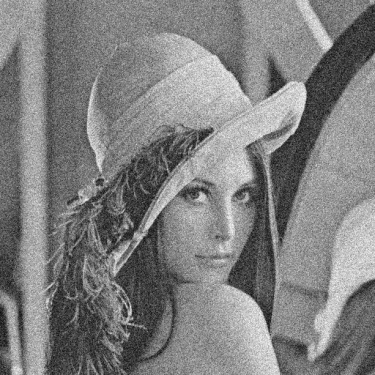
\includegraphics[width=.4\linewidth]{img/preprocessing/denoise_orig.png}
&
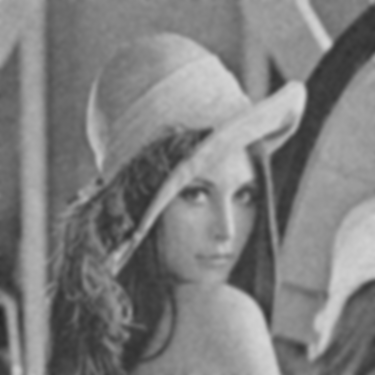
\includegraphics[width=.4\linewidth]{img/preprocessing/denoise_gauss.png}
\vspace{1em} \\
Median filter & Non-local means method \\
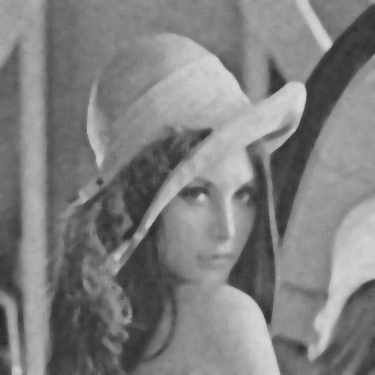
\includegraphics[width=.4\linewidth]{img/preprocessing/denoise_median.png}
&
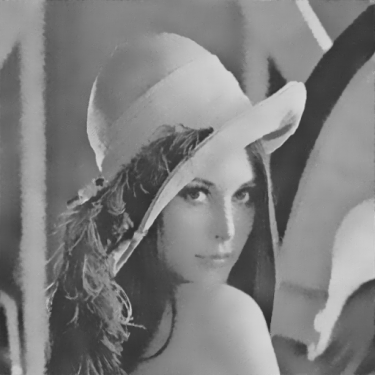
\includegraphics[width=.4\linewidth]{img/preprocessing/denoise_nonlocal.png}
\end{tabular}
}
\caption{Comparison of denoising techniques}
\label{fig:preprocessDenoising}
\end{figure}

What combination of techniques to use for the optimal results greatly depends on the input image --- if there is little to no noise, denoising an image can cause more harm than good. Therefore, it is always important to approximately compute the signal:noise ratio before applying any kind of filters.

Determining the presence of noise is a complex task. Although simple heuristic algorithms (based on finding differences between adjacent pixels) have been tested for these purposes, they rendered poor results and had a visibly high execution time. Therefore, more complex solutions requiring knowledge in the field of probability and statistics, specifically probability distribution, have been tested~\citep{noiseDetection}. These are based on the idea of separating frequencies, and render quite satisfactory results. However, as these methods might still fail at specific images, the user is advised to determine the presence of noise manually.

\subsection{Scanning border reduction}

Scanned documents often have visible dark borders (\emph{marginal noise}). These are created either during scanning (due to the presence of neighbouring pages) or are an unwanted result of the binarization process.

As performing a scanning border removal might be harmful in case there was no marginal noise present, this process has two steps --- marginal noise detection and, if successful, marginal noise reduction.

Marginal noise is present as a dark connected component of the page. This is a fact that most detection algorithms take advantage of. Firstly, they extract the connected components of the page. This can be done for example by a \emph{black filter} (a moving rectangular window that calculates the ratio of black pixels on border~\citep{marginalNoiseWindow}). After obtaining the connected components, different heuristics are used --- most based on removing the connected components near the edges. In the end, usually a "cleanup" is performed (like \emph{white filter}~\citep{marginalNoiseWindow}) for removal of all unnecessary elements around the borders (an unwanted text from the neighbour page, noisy components in the corners\ldots).

The results of this algorithm depend greatly on the values of thresholds, margins and other hard coded parameters. This is why the cleanup part's parameters are usually dependant on the results of previous parts of this process.

Another approach is the one mentioned by \citet{marginalNoiseEdge}. It is based on edge density calculations, and the fact that text areas have generally a much lower density than edge areas. An edge detector (in this case, \emph{sobel}) is used for examining vertical marginal noise, and later horizontal marginal noise. It returns the positions of the margins. Anything beyond these positions is detected as an unwanted noise, and can be therefore removed by filters or other removal algorithms.

\begin{figure}
\centering

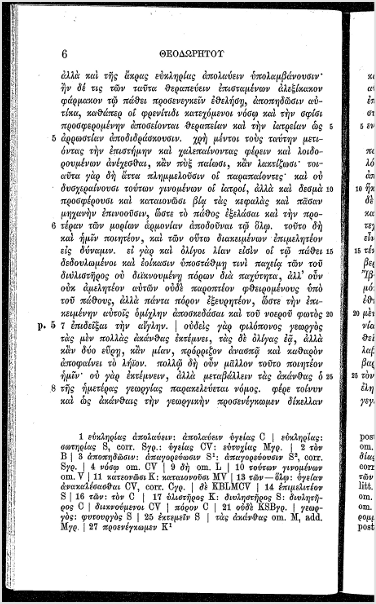
\includegraphics[height=10em]{img/preprocessing/scan_borders_orig.png}
\qquad
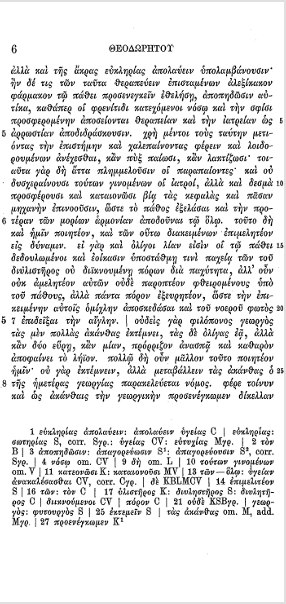
\includegraphics[height=10em]{img/preprocessing/scan_borders_result.png}

\caption{Removal of scanning artifacts. Left: original, right: removed scanning borders.}
\label{fig:scanning}
\end{figure}

\section{Text detection process}

There exist two main approaches for text detection in OCR. The first one is an approach based on heuristics. It includes techniques of page segmentation, line and element detection and character detection, which are based on different approximations and sometimes naive algorithms. The second one is an approach that is widely used and researched today --- and that is the use of neural networks.

In this paper, we will be concentrating on the heuristics approach of the OCR problem, as we use it in our implementation. However, neural network recognition is a promising field of study and also deserves a mention.

Although OCR engines greatly differ in the way their heuristic approaches work, they all contain the following steps:
\begin{enumerate}
    \item \emph{Page segmentation} --- logical and topological division of the page into multiple smaller segments
    \item \emph{Representation and feature extraction} --- simplification of the extracted elements of the image for improvement of the OCR accuracy and execution time
    \item \emph{Character classification}
\end{enumerate}

We analyze these steps in the following individual subsections.

\subsection{Page segmentation}

The idea behind the page segmentation process is to obtain page blocks that contain individual characters. This, however, is not always possible due to the errors that occur during this process, which result in either merging or splitting the characters. Therefore, in OCR engines, page segmentation process usually means any kind of logical or topological division of the image into multiple smaller blocks --- which can be either characters, lines or even paragraphs.

Page segmentation can be performed in three different ways~\citep{segmentationBenchmark} --- either we start with an image as a whole and recursively divide it into parts until certain criterion is met (top-down), or we start with individual pixels and group them according to similarity of their attributes (bottom-up), or we use a combination of these two methods.

\subsubsection{Page segmentation techniques}

In this section, we present a few concrete algorithms widely used for heuristic page segmentation.

\xxx{co ta tabulka?}

\xxx{TO DO - chcem dat captions tym fboxom, netusim vobec ako}

\clearpage

\begin{longtable}{p{7em}p{13em}c}
\toprule
\textbf{Page} & \textbf{Description} & \textbf{Image} \\
\textbf{Segmentation} & & \\
\textbf{Algorithm} & & \\
\midrule
RXYC

algorithm

(\emph{X-Y cut})
&

one of the oldest and simplest methods

tree based algorithm, works by recursively splitting the nodes of the tree into rectangular parts

uses projection profile and threshold computations for determination of splitting

easy to implement, fast

usually fails at the presence of imperfections

&
\fbox{\raisebox{-\height}{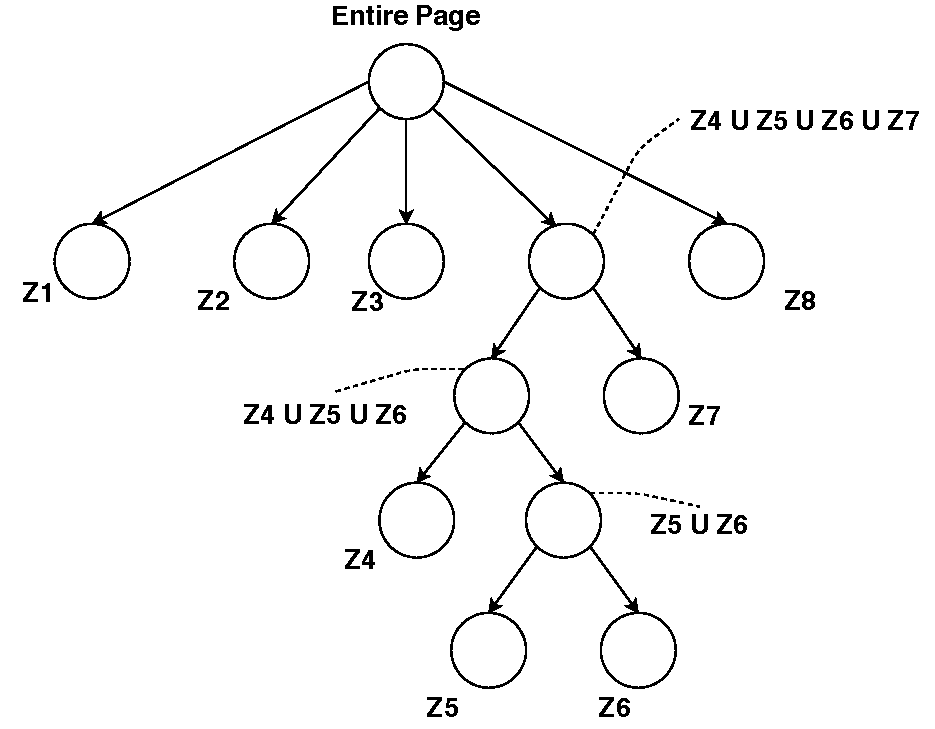
\includegraphics[width=0.3\textwidth,
height=40mm]{img/textDetection/segm_rxyc.pdf}}}\\
Smearing 

algorithm 

(\emph{RLSA})
&

based on linking together black areas that are no more than C pixels away from each other

requires binarized images

slightly better results than \emph{X-Y cut}

fails at the presence of noise, not used for text documents

widely popular among vehicle plate recognition
 &
\fbox{\raisebox{-\height}{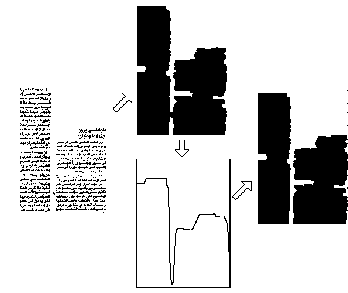
\includegraphics[width=0.3\textwidth,
height=40mm]{img/textDetection/segm_smearing.png}}}\\
Voronoi

diagram 

based

algorithm&

bottom-up algorithm

performs a noise removal 

creates Voronoi diagram from sample points of edges of extracted connected components of the existing image

performs a "clean-up" of the diagram - deletion of superfluous edges

can be used on documents with noise and other imperfections

causing over-segmentation errors when working with documents using different fonts or styles

advised to use on homogeneous collection of documents &
\fbox{\raisebox{-\height}{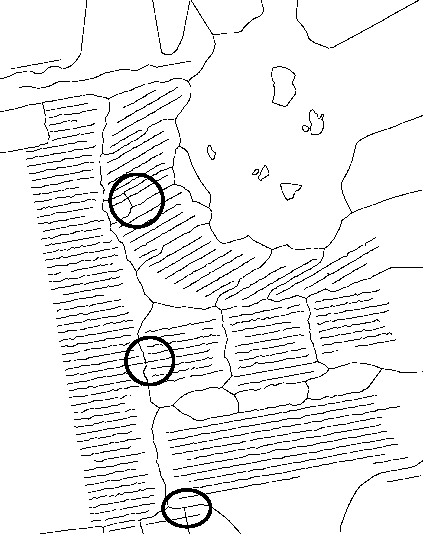
\includegraphics[width=0.3\textwidth,
height=60mm]{img/textDetection/segm_voronoi.png}}}\\
Docstrum

algorithm

&

bottom-up algorithm

based on fonts and styles of the characters

divides connected components into a dominant font group and a group with characters from titles or sections heading

performs a near-neighbor clustering of components in each group

determines the skew of the image and text-lines, upon which merges within-line nearest neighbor pairs into text-lines and blocks

similar errors like \emph{Voronoi diagram} algorithm

advised to use on a homogeneous collection of documents
&
\fbox{
\raisebox{-\height}{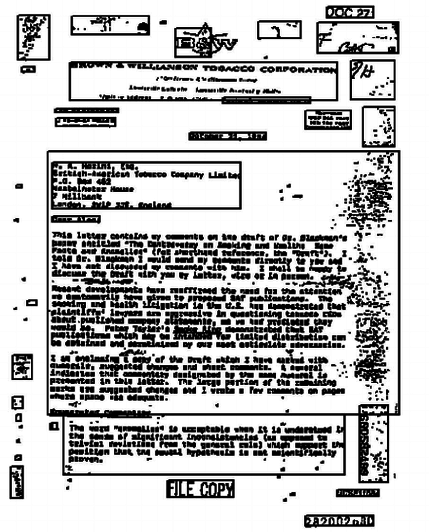
\includegraphics[width=0.3\textwidth,
height=60mm]{img/textDetection/segm_docstrum.png}}}\\
Whitespace

analysis

&

assumes a white background of the image

finds a union of white rectangles as a cover of the background

uncovered regions of the image after applying the union are the results of segmentation

satisfactory results on heterogeneous documents

tends to result in either over-segmentation or under-segmentation depending on the sizes of rectangles in the union

overall, performs worse than \emph{Voronoi} or \emph{Docstrum} algorithm
&
\fbox{
\raisebox{-\height}{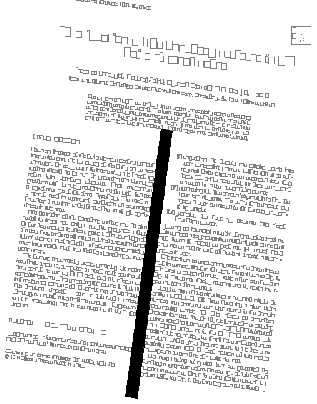
\includegraphics[width=0.3\textwidth,
height=60mm]{img/textDetection/segm_whitespace.png}}}\\
Constrained

text-line

detection
&

similar to \emph{whitespace analysis}, differs in the approach of finding the whitespace rectangles that cover the page background

good option for documents with different font sizes or layouts

nearly parameter free
&
\fbox{
\raisebox{-\height}{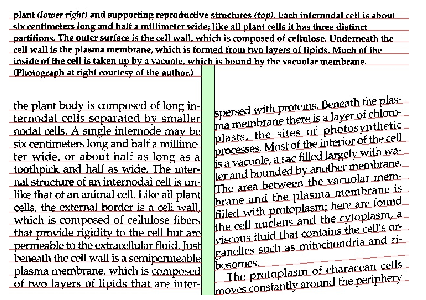
\includegraphics[width=0.3\textwidth,
height=60mm]{img/textDetection/segm_textline.png}}}\\
\bottomrule
\caption{Page segmentation algorithms}
\label{tab:segmentationOverview}
\end{longtable}

\subsubsection{Tesseract page segmentation} \label{sectionTessPageSegm}

Another slightly different segmentation technique was proposed by~\citet{tesseractSegmentationTab}. This method is based on detecting so-called \emph{tab-stops}.

\emph{Tab-stops} are used in word processors to enable correct and eye pleasing alignment of text, and are present in the document as margins, column edges, indentations. All of them are placed at fixed x-positions at which edges or centers of text lines are vertically aligned.

The process of page segmentation by tab-stops has multiple steps. It begins by searching the document image for connected components. By grouping these connected components into vertical lines and examining their vertical alignment, tab-lines are then detected. Based on these tab-lines, connected components of the page layout analysis are then grouped into \emph{column partitions}, which do not cross any tab-lines and are of the same type. In the end, a few of the column partitions can be merged or divided into segmented blocks, based on different types of fonts or line spacing. 

This method is implemented and used by the Tesseract engine, with the preprocessing help of the Leptonica library. It claims to yield satisfactory results (presented in~\cref{fig:segmentationTesseract}, given the input document is properly preprocessed.

\begin{figure}
    \noindent
	\makebox[\textwidth]{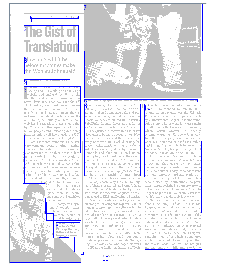
\includegraphics[width=20em]{img/textDetection/segm_tabstop.pdf}}
	\caption{Tesseract engine segmentation}
	\label{fig:segmentationTesseract}
\end{figure}

There exist many other segmentation methods that approach this problem differently. For example, with segmentation of scanned books that mostly have Manhattan layout, a simple deskewing and horizontal and vertical cuts should suffice. Also, algorithms focusing on recipe or ticket analysis already know what the approximate layout of the received image will be. They can therefore simplify these complicated algorithms for their purposes.

\subsection{Representation and feature extraction}

Upon extracting elements by page segmentation, we are left with an unnecessary amount of information. Trying to run a text recognition algorithm on all of it would be significantly time consuming. Additionally, as the character recognition is based on specific features for each symbol, the extra information might not suit the character features of the correct candidate. Therefore, the candidate gets undesirably discarded, which results in decreased accuracy.

For these reasons, a set of features is extracted for each element that distinguishes it from other element classes while keeping characteristic differences. There exist various different features, generally divided into local features, which are usually geometric (like number of endpoints of each character, convex or concave parts, branches etc.), and global features, which are usually topological (connectivity, number of profiles, number of holes\ldots). The set of features that will represent each characters needs to be picked carefully, so that they define the shape of a character precisely a uniquely but are also the smallest set possible to prevent increased memory usage and time complexity.

There exist three methods for performing feature extraction, described by both~\citet{featureExtractionBook} and~\citet{featureExtractiontext}. They differ in the ways the features are derived from the character, in reconstructability (whether the image can be reconstructed to its previous version solely from its features), in invariance to transformations and many more. We describe these methods in the following list:

\begin{itemize}

\item \emph{Global transformation and series expansion}

These include methods like Fourier or Gabor transform, Fourier Descriptor, Wavelets, Moments and Karhunen-Loeve expansion, and are based on the representation of continuous signals by a linear combination of simpler functions. The coefficients of the linear combination provide a compact encoding known as transformation or series expansion. Therefore, deformations like translation and rotations are invariant under these methods. However, the downside of these approaches is the time complexity, as these methods require a number of non-trivial computations.

\item \emph{Statistical representation}

Unlike transforms, these features are based on the statistical distribution of points in an element. They provide high speed and low complexity and also take care of different font and style variations to some extend. Methods based on this representation are e.g. \emph{zoning} (where the frame containing the character is split into different zones, which are then analyzed for densities of points and strokes), \emph{crossings and distances} (crossing --- the number of crossings of the character along vertical and horizontal lines; distances --- the distances of character pixels from frame boundaries), and other like projections, characteristic loci etc. We present a few of these techniques in~\cref{fig:featureExtractionStatistical}.

The downside of this approach is the invariance to transforms --- if the character is only slightly skewed, the feature extraction results will greatly differ.

\item \emph{Geometrical and topological representation}

These features are based on the geometrical and topological properties of the individual elements, like basic line types that form a character skeleton. They also include features of the character contour like extreme points, maxima, minima, cross points, line ends, isolated dots, different types of strokes and many more. We present a few of them in~\cref{fig:featureExtractionGeometrical}.

They highly tolerate various distortions and style variations, and their output can be assigned into a feature extraction vector.

\end{itemize}

We present a few sample examples of feature extraction techniques in~\cref{fig:featureExtraction}.

In conclusion, the goal of any representation and feature extraction technique is to create a "skeleton" for each character by selecting the most representative information from the raw data which maximizes the recognition rate with the least amount of elements. 

\begin{figure}[t]
\centering
{\sffamily
\begin{tabular}{cc}
Zoning & Crossing and distances~\citep{crossingAndDistances}\\
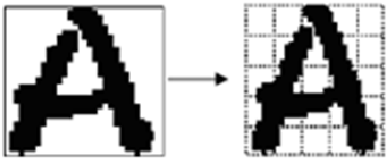
\includegraphics[height=6em]{img/textDetection/feature_zoning.png}
&
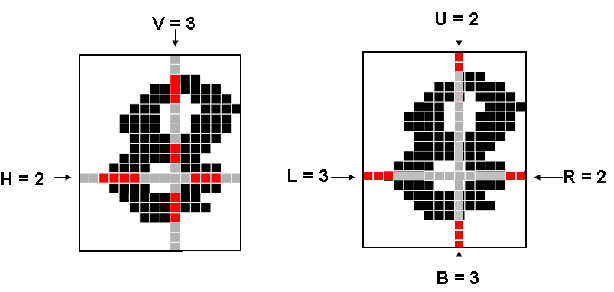
\includegraphics[height=6em]{img/textDetection/feature_crossing.png}
\end{tabular}
}
\caption{Examples of feature extraction techniques}
\label{fig:featureExtractionStatistical}
\end{figure}

\begin{figure}[t]
\centering
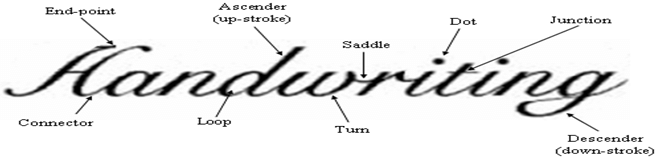
\includegraphics[width=0.8\linewidth]{img/textDetection/features_geometrical.png}
\caption{Example of a few geometrical and topological features~\citep{geometricalFeatures}}
\label{fig:featureExtractionGeometrical}
\end{figure}


\subsection{Character classification}
\todo{Trosku problem je, ze na relativne jednoduchy metody pripravy textu spotrebujes 15 stranek a o hledani a klasifikaci pismen mas 1 sekci.}

OCR engines widely use the methodologies of pattern recognition, which assign an unknown sample into one of its predefined classes. These approaches are not necessarily independent of each other and OCR engines frequently combine subsets of them to achieve the most accurate results.

One way to approach classification is by \emph{template matching}~\citep{templateMatching}. It is based on the existence of predefined \emph{templates} --- multiple bitmaps containing characters of the alphabet. Improved version of this method have an extended database of templates, including numbers and special characters. Once a character is detected, it is passed to the algorithm and for every existing template, its similarity ratio is calculated. The template with the greatest ratio is then assumed to be the recognized character. This method has various implementation depending on how the ratio is calculated --- for example, cross correlation, normalized correlation or euclidean formula can be used.

Although the implementation of this method is very simple, even small disfigurements and noise can greatly affect its efficiency. Also, in this case, a feature extraction would be unnecessary as all templates are created manually. We present this technique in~\cref{fig:characterClassTemplate}.

\begin{figure}[t]
    \noindent
	\makebox[\textwidth]{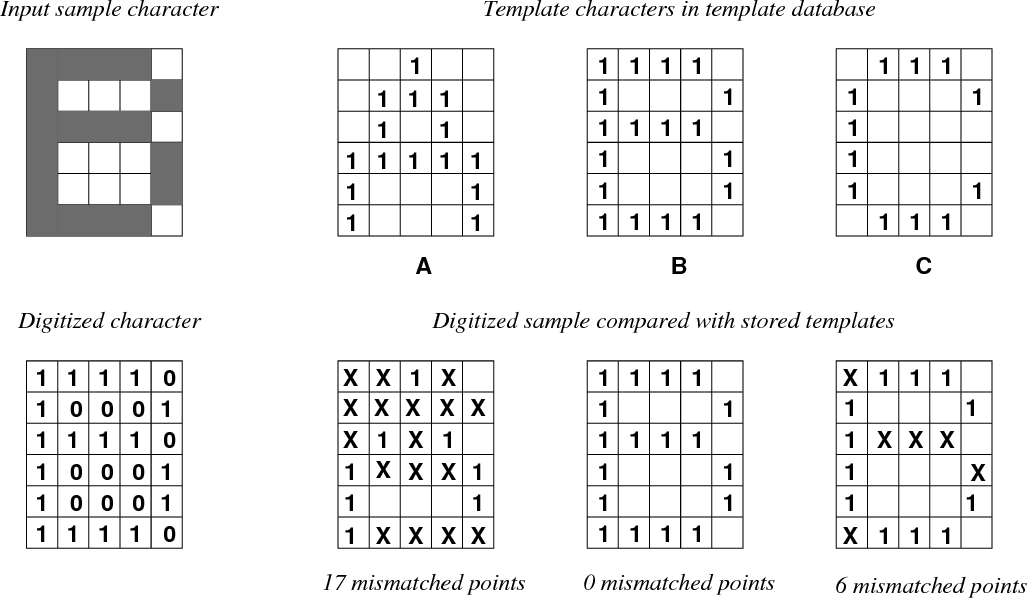
\includegraphics[width=30em]
	{img/characterClassification/templates.png}}
	\caption{Examples of template matching technique as described by~\citet{Ning1993AnIO}}
	\label{fig:characterClassTemplate}
\end{figure}

Another approach is by using \emph{statistical techniques}~\citep{characterClassification}, like Bayes classifier, Hidden Markov Modeling or Nearest Neighbor. These techniques are based on feature extraction for each character. To classify an unknown character, its extracted features are compared to the features of training data with the help of statistical decision function. 

The problem with these algorithms is that they have no information about whole-part relations. We present the possible extracted features for these techniques in~\cref{fig:characterClassificationStatis}.

\begin{figure}[t]
\centering
{\sffamily
\begin{tabular}{ccc}
Existence and number & Number of & Number of \\
of end points & vertical lines & horizontal lines \\
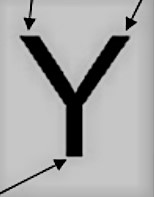
\includegraphics[height=10em]{img/characterClassification/statis_endPoint.jpg}
&
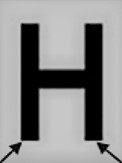
\includegraphics[height=10em]{img/characterClassification/statis_vertical.jpg}
&
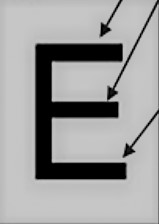
\includegraphics[height=10em]{img/characterClassification/statis_horizontal.jpg} \\
\end{tabular}
}
\caption{A few of the possible extracted features in statistical techniques~\citep{vithlani2015structural}}
\label{fig:characterClassificationStatis}
\end{figure}

For this reason, a newer approach has been tested out over the past few years --- \emph{machine learning}~\citep{characterClassification}.

\emph{Machine Learning}~\citep{sebastiani2002machine} is a method of data analysis based on artificial intelligence. Over time, it builds models of "training data". Based on them, it makes decisions and predictions on its input. 

In the case of character classification, training data is created by passing various characters into the engine along with their correct output. In this way, the engine learns how different characters should look and applies this knowledge to its input.

This method is for example used in a one of the simplest machine learning algorithms, and that is the \emph{KNN classification algorithm} (or K-Nearest neighbor algorithm), which we present in~\cref{fig:characterClassKNN}. The input image is compared to the training data and chooses its K nearest objects (objects that are the most similar). After that, the image is classified with being assigned to the class most common among its K nearest neighbors.

\begin{figure}[t]
\centering
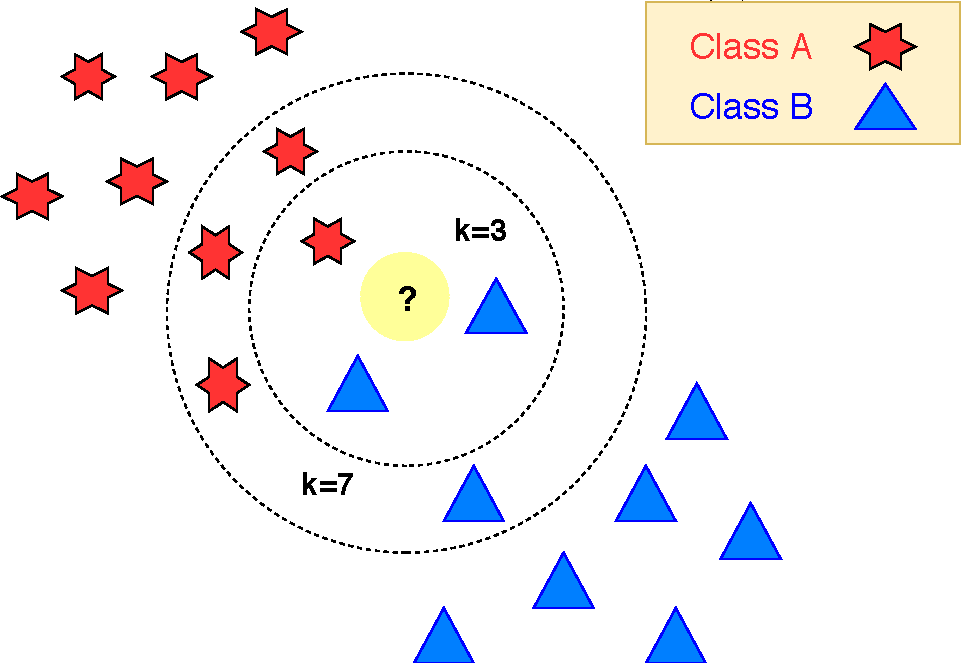
\includegraphics[width=0.7\linewidth]{img/characterClassification/knn.pdf}
\caption{KNN algorithm: with k=3, the algorithm will assign the new element to class A; with k=7 to class B } \label{fig:characterClassKNN}
\end{figure}

More complex methods include the \emph{Support Vector Machine algorithm} (SVM). This approach divides its received data into two classes --- training and testing data. The goal of SVM technique is to deliver a model that predicts the output of the test set.

The learning is done by a \emph{SVM kernel}. The kernel is, briefly speaking, a combination of mathematical function that takes two inputs and returns an information about how similar they are. Other than kernel functions, there are other parameters that tune the output of the SVM algorithm, presented in~\cref{fig:characterClassSVM} --- \emph{margin} parameter tells the engine the separation of line to the closest class points, \emph{gamma} parameter decides how far the influence of a single training example reaches and \emph{regularization} parameter controls the misclassification of elements.

\begin{figure}[t]
\centering
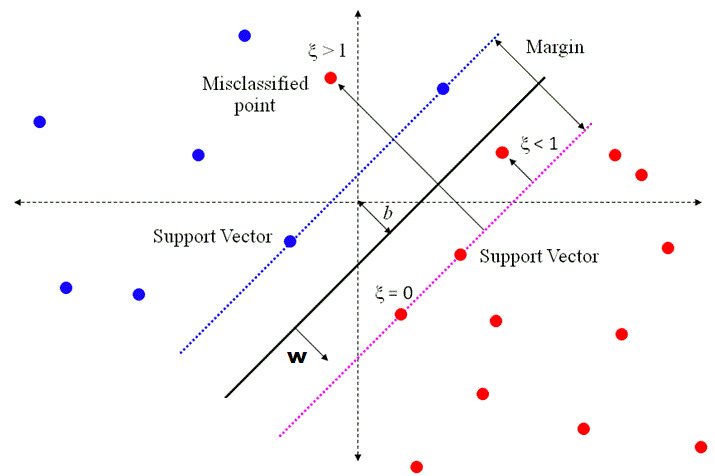
\includegraphics[width=0.7\linewidth]{img/characterClassification/svm.jpg}
\caption{The process of determination of classes in SVM algorithm~\citep{svmAlgorithm}}
\label{fig:characterClassSVM}
\end{figure}

Many experiments have been executed in the field of machine learning for character classification. However, none of them can guarantee the accuracy of different approaches, as they all greatly depend on the training data. The more training data is provided to the machine, the more accurate its recognition is. 

\section{Available OCR software}

OCR engines greatly differ not only in the accuracy of their recognition, but also in the features that they provide. Although OCR engines focusing only on text recognition exist, most of the modern software contains recognition of other document elements, like images, forms, tables and many more. Further differences include the presence of preprocessing options, support for various file extensions, recognition of different fonts, including handwritten documents, and many more. Furthermore, there exist OCR engines specialized in processing only specific types of images, such as automatic number plate recognition engines or ticket validation engines.

In~\cref{tab:availableSoftware}, we present the most popular and widely used free OCR engines. Commercial software used for the purposes of OCR, such as ABBYY FineReader, Readiris and OmniPage, also deserves a mention. However, although some of these engines produced overall better results than the free software, it is unusable for the purposes of this thesis.

\begin{table}[t]
{\small
\begin{tabular}{p{4.6em}p{2em}p{3em}p{4.8em}p{7em}p{7em}}
\toprule
\textbf{Name} & \textbf{Year} & \textbf{Code} & \textbf{Languages} & \textbf{Features} & \textbf{Notes}\\
\midrule
Tesseract & 1985 & C++, C & 100+ & 
layout analysis

detection of different elements

right-to-left processing

&

both neural networks and heuristics

command line interface

\\
Ocrad & 2003 & C++ & Latin alphabet &  
layout analyser

command line interface
&
can read only 3 different formats
\\
GOCR & 2000 & C & 20+ &

translates barcodes

command line interface

&
failure at heterogeneous fonts

\\
CuneiForm & 1996 & C, C++ & 28 & 

used for scanned documents

batch conversion

& 
results almost always need postprocessing

\\
OCRopus & 2007 & Python & Latin script & 

engages neural networks

can be improved by training

\\

\bottomrule
\end{tabular}
}
\caption{Overview of available OCR software}
\label{tab:availableSoftware}
\end{table}

\subsection{Tesseract}

Originally developed by Hewlett-Packard Company around 1990~\citep{TesseractGIT}, Tesseract is one of the most robust and accurate open-source OCR engines. When it was firstly developed, Tesseract could only accept TIFF images containing simple one-column text in English language. Since then, it has undergone a lot of improvements and added many features. As of today, Tesseract supports multi-columned documents (via its page-layout analysis), claims to support over 100 languages (including right-to-left text such as Arabic or Hebrew), works on different input and output image formats (with the help of Leptonica~\citep{LeptonicaLIB} library) and is available for Windows, Linux and even Mac OS. In its latest version (4.0.0), Tesseract also added a new neural network (specifically a LSTM network) focused on line recognition. 

Tesseract does not have a GUI and works as a command line program. It is used mostly for development purposes and provides an OCR engine (libtesseract) that gives developers a chance to create their own applications using tesseract API. Also, Tesseract contains no preprocessing algorithms. It advises users preprocess the input images themselves~\citep{TesseractQual}.

This is the reason why many wrappers and other 3rd party projects using Tesseract have been created. These projects mostly focus on creating GUIs for Tesseract or adding preprocessing algorithms to make the Tesseract engine more user-friendly. Although Tesseract is still in the process of development, it plans on doing no such thing and its future work consists mainly on focusing on LSTM networks.

Tesseract is one of the few OCR open-source engines. Based on our observation, it provides the most features and in general cases, provides the best accuracy of element recognition amongst all the other open-source OCR engines. Moreover, we found its documentation, information accessible about individual functions and even examples of use cases well-arranged and easy to understand.

This is the reason why we use the recognition and features of this engine in our implementation.

\subsubsection{Tesseract character recognition}

In this section, we present an overview of the way Tesseract (and therefore, we) detects various lines containing text (\emph{textlines}) and symbols. Thoroughly analyzed by~\citet{smith2007overview}, this algorithm has the following steps:

\begin{enumerate}
    \item \emph{Page layout analysis}
    
    Already discussed in~\cref{sectionTessPageSegm}, page layout analysis is the first and one of the most crucial steps in an OCR algorithm. Line detection relies on this step to provide meaningful text regions.
    
    \item \emph{Line finding}
     
     Upon obtaining text regions, heuristics like height filter and median filter are used to estimate the height of characters and remove noise, punctuation and other obstacles. The filtered so-called \emph{blobs} are then merged into lines by their y-coordinate and position.
     
     The problem that occurs in this step is the sloping of the blobs when the lines are skewed. Tesseract tries to solve it by sorting the blobs by their x-axis --- therefore, firstly unique lines will be created, and then other blobs will be added to these lines while tracking the slope across the page.
     
     Once the blobs are assigned to lines, they are merged based on heuristic criterion.
     
     \item \emph{Baseline fitting}
    
    The next step is to find a baseline for each line, as shown in~\cref{fig:textRecTesseractBaseline}. These baselines are fitted using a quadratic spline, as curved baselines can also be present.
    
    \item \emph{Character chopping}
    
    Upon determining lines, Tesseract tries to chop the existing words into characters. This is done pretty easily when handling fixed-pitch text --- Tesseract simply chops the word into individual characters by the determined pitch. Complications arise with the presence of non-fixed-pitch text~\cref{fig:textRecTesseractSpacing}. In this case, Tesseract tries to determine the size of a character by measuring the gaps between baseline and the upper boundary of the characters. In case it is unsure of its decision, then the final decision can be made after word recognition.
    
    \item \emph{Word recognition}
    
    This step is applied only to non-fixed-pitch text, as the fixed-pitch is already properly segmented into words. As the results from the previous step might have been unsatisfactory with a few missing chops, this step proceeds to further chop blobs according to various heuristics. Firstly, candidate chop points are found from concave vertices of a polygonal approximation of the outline. Based on heuristics, a few of these candidate chops are then performed, with the number of them being higher than the actual chops needed. Therefore, broken characters (characters that have been chopped more times than they should have) are repaired by an \emph{associator} that already has knowledge of existing characters. It uses this knowledge to find the best-first combination of chopped blobs to merge into candidate characters.
    
    \item \emph{Character classification}
    
    The last thing on the list is the actual character classification. Earliest versions of Tesseract used a static character classifier based on topological features. However, this approach was not robust to damaged characters in real-life images. This was solved by extracting multiple small features of fixed length from the unknown and merging them to match more robust features of a character, as presented in~\cref{fig:textRecTesseractChars}.
    
    Classification itself is then performed by matching the characters to a training data set and outputting the character that has the greatest number of similar features (where the \emph{greatest number} computation is based on heuristics).
    
\end{enumerate}

\begin{figure}[t]
\minipage{\textwidth}
    \centering
    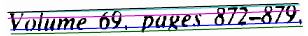
\includegraphics[width=0.7\linewidth]{img/textDetection/tesseractBaseline.png}
    \caption{An example of a fitted baseline(dark blue) along with helper lines used for baseline fitting and later, character chopping~\citep{smith2007overview}}
    \label{fig:textRecTesseractBaseline}
\endminipage\hfill
\minipage{0.45\textwidth}
    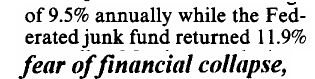
\includegraphics[width=\linewidth]{img/textDetection/tesseractSpacing.png}
    \caption{Non-fixed pitch text spacing issues~\citep{smith2007overview}}
    \label{fig:textRecTesseractSpacing}
\endminipage\hfill
\minipage{0.45\textwidth}
    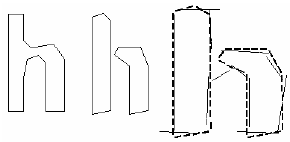
\includegraphics[width=\linewidth]{img/textDetection/tesseractCharacters.png}
    \caption{Left: original letter h; middle: broken character; right: merging of multiple smaller features~\citep{smith2007overview}}
    \label{fig:textRecTesseractChars}
\endminipage
\label{fig:textRecTesseract}
\end{figure}